\section{Forecast Error vs. Lead Time (Q2)}\label{sec:leadtime}

In this section, we examine how forecast errors change over lead time and by how much. To achieve this, we computed and observed the MAE, RMSE, MAPE, and error growth rates across lead times.

\subsection{Error metrics across lead time}

Figure~\ref{fig:leadtime} shows MAE, RMSE, and MAPE as a function of lead time for each of the
eight variables, pooled over all \num{896} sites and all three years.

\begin{figure}[H]
  \centering
  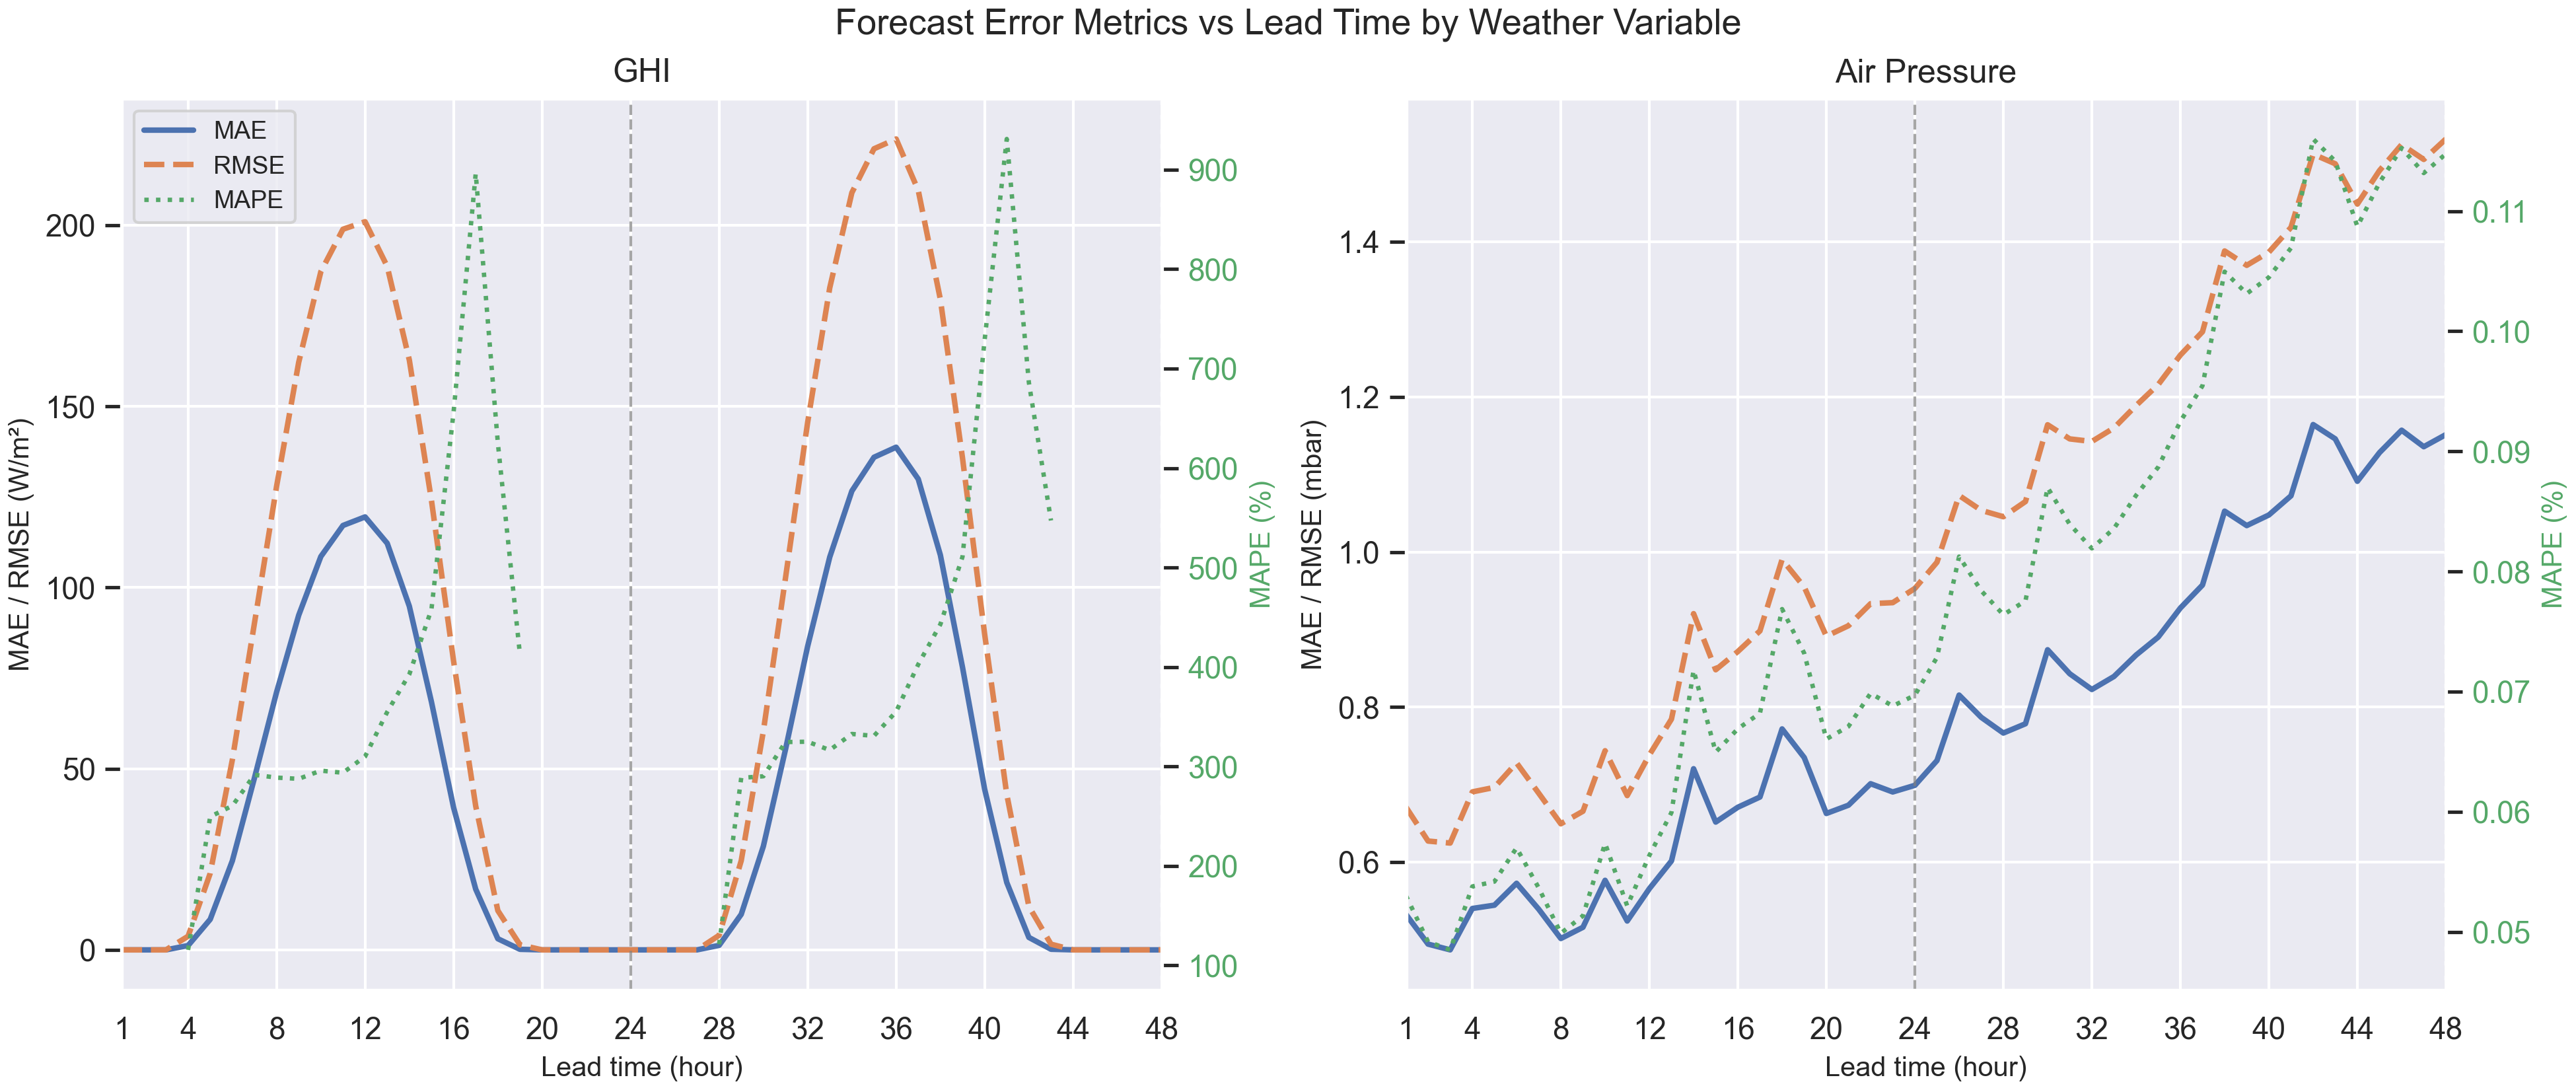
\includegraphics[width=\textwidth]{figures/Q2/embed/error_by_lead_time_ghi_pressure copy.png}
  \caption{Forecast error metrics versus lead time, by variable. MAE (solid) and RMSE (dashed)
  are on the left axis in native units; MAPE (dotted) is on the right twin axis in percent.
  MAE and RMSE generally grow with lead time and show twin peaks near lead~12 and~36---the
  diurnal signature created by the fixed \texttt{06z} init (those leads fall near solar noon).
  RMSE $\ge$ MAE throughout, with the gap widening slightly, indicating that larger errors
  become relatively more frequent further out. GHI rises from and returns to $\approx 0$ twice
  (it is $\approx 0$ at night); its MAPE is unstable, so MAPE is only interpretable for pressure
  and relative humidity.}
  \label{fig:leadtime}
\end{figure}

The key observations are: (i) MAE and RMSE rise with lead time and (ii) exhibit two diurnal peaks at
roughly leads 12--16 and 36--40; (iii) RMSE exceeds MAE throughout and the gap widens slightly with lead,
implying that forecast stability drops as the horizon grows; and (iv) MAPE is only meaningful
for pressure and relative humidity---for the other variables the small or zero denominators
inflate it beyond use. The exception to (i) is GHI because irradiance drops to 0 at night, and the exception to (ii) is air pressure, as its plot shows several oscillations instead of two diurnal peaks.

\subsection{Error growth rate}

We define the \emph{error-growth rate} as the change in the error between
consecutive lead hours, $\Delta\text{Error}/\text{hr}$. Figure~\ref{fig:growthcurves} shows the
fleet-mean growth curve per variable, and Figure~\ref{fig:growthdist} shows the box plot distributions of the error growths for each lead time.

\begin{figure}[H]
  \centering
  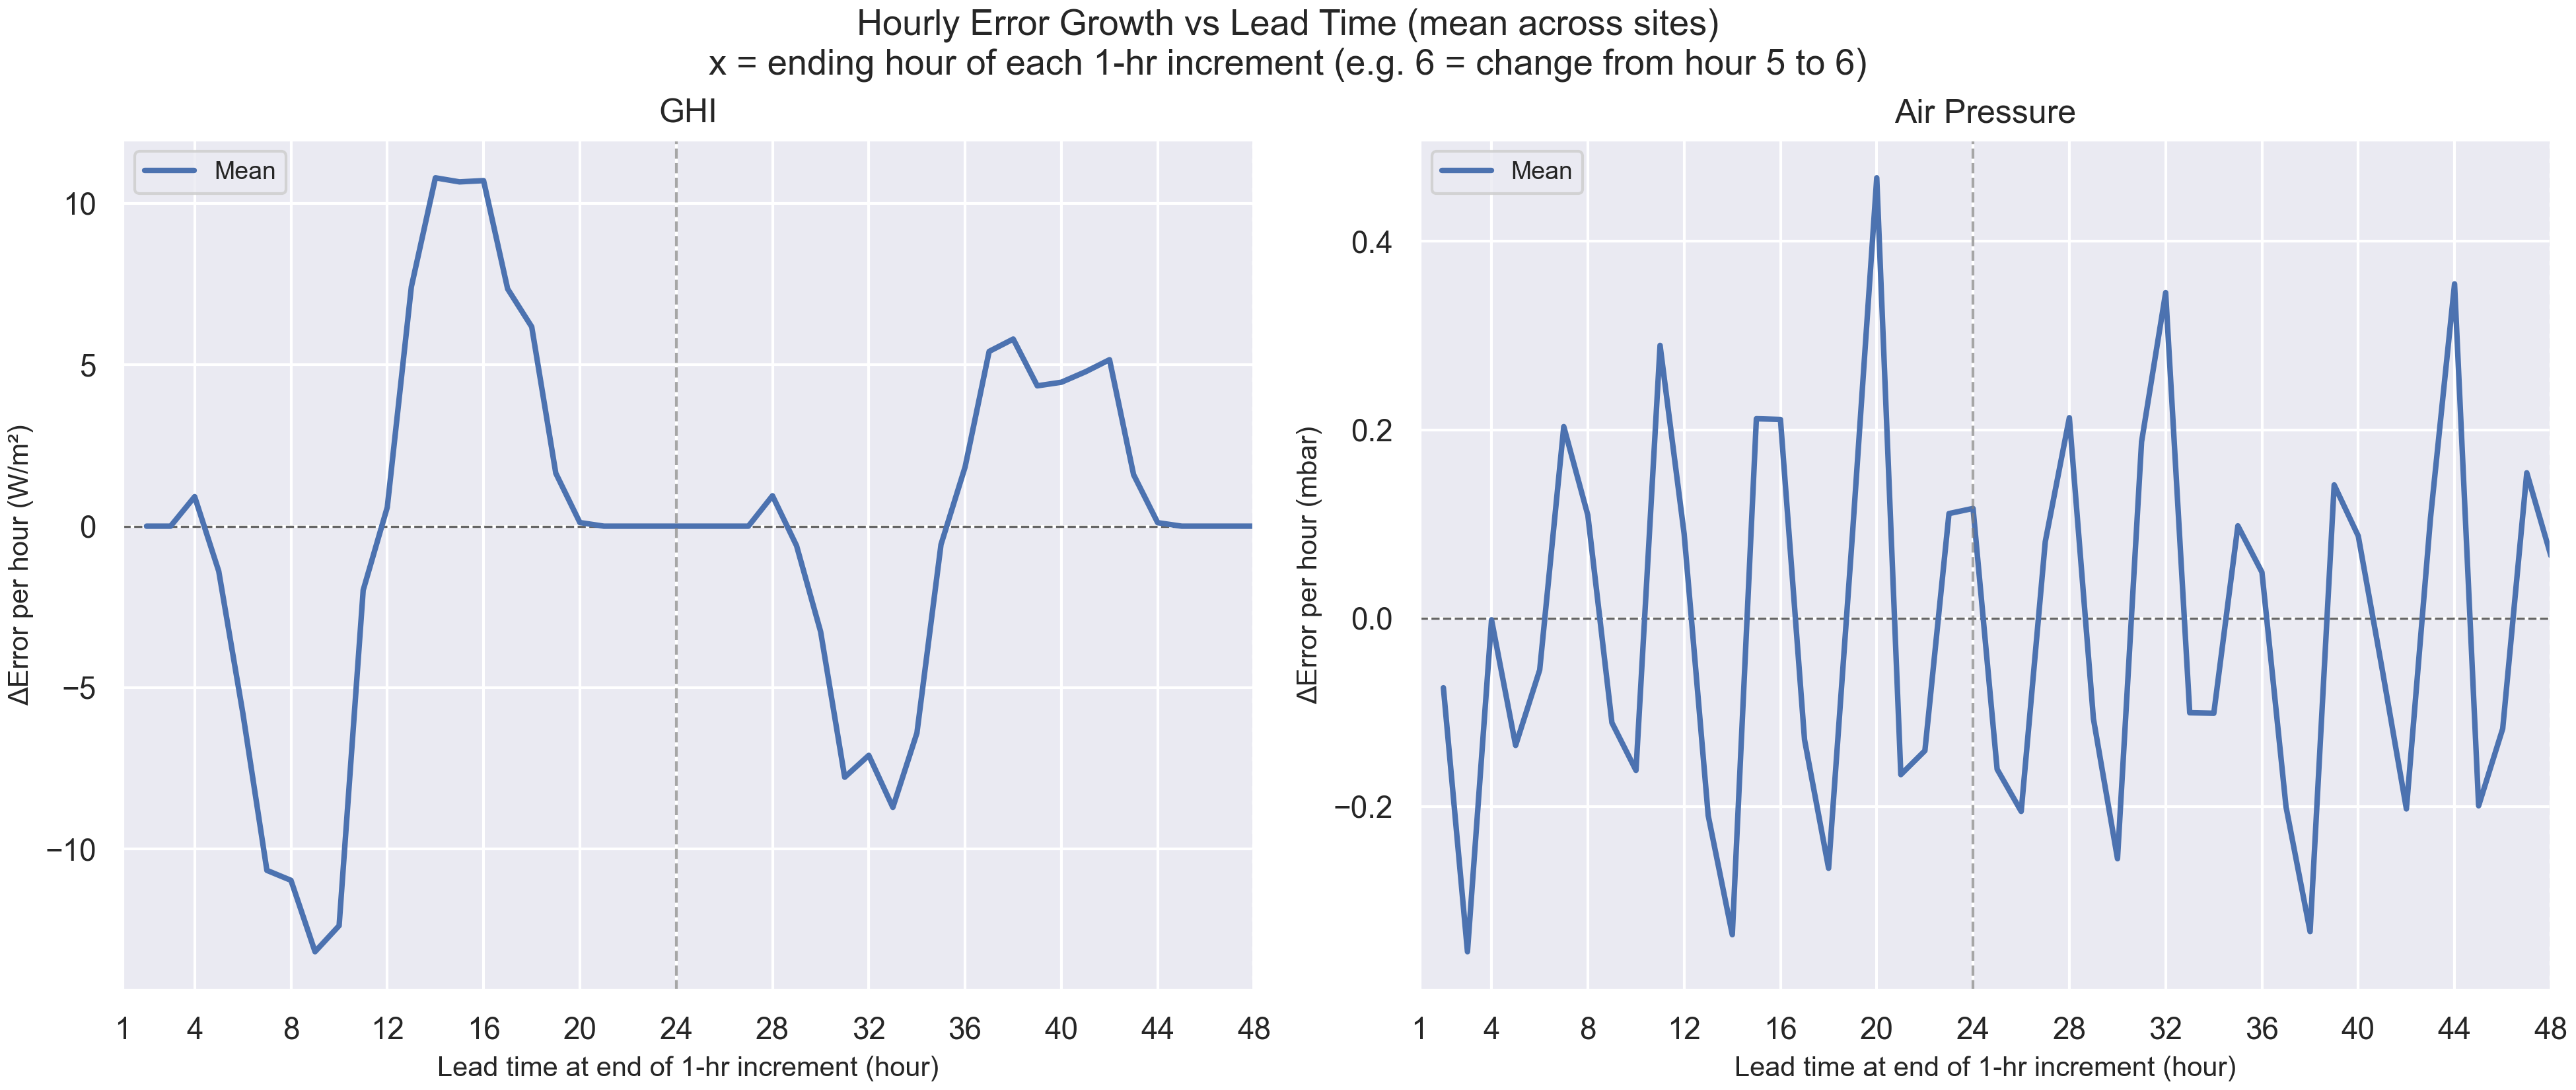
\includegraphics[width=\textwidth]{figures/Q2/embed/error_growth_curves_ghi_pressure copy.png}
  \caption{Fleet-mean hourly error-growth rate ($\Delta\text{Error}/\text{hr}$) versus lead time.
  GHI traces a clear diurnal sinusoid (least volatile near sunrise/sunset); the other variables
  hover around zero with no obvious trend, and pressure is the noisiest. Curves oscillating
  around zero---rather than staying positive---indicate that bias does not drift monotonically
  with lead time.}
  \label{fig:growthcurves}
\end{figure}

\begin{figure}[H]
  \centering
  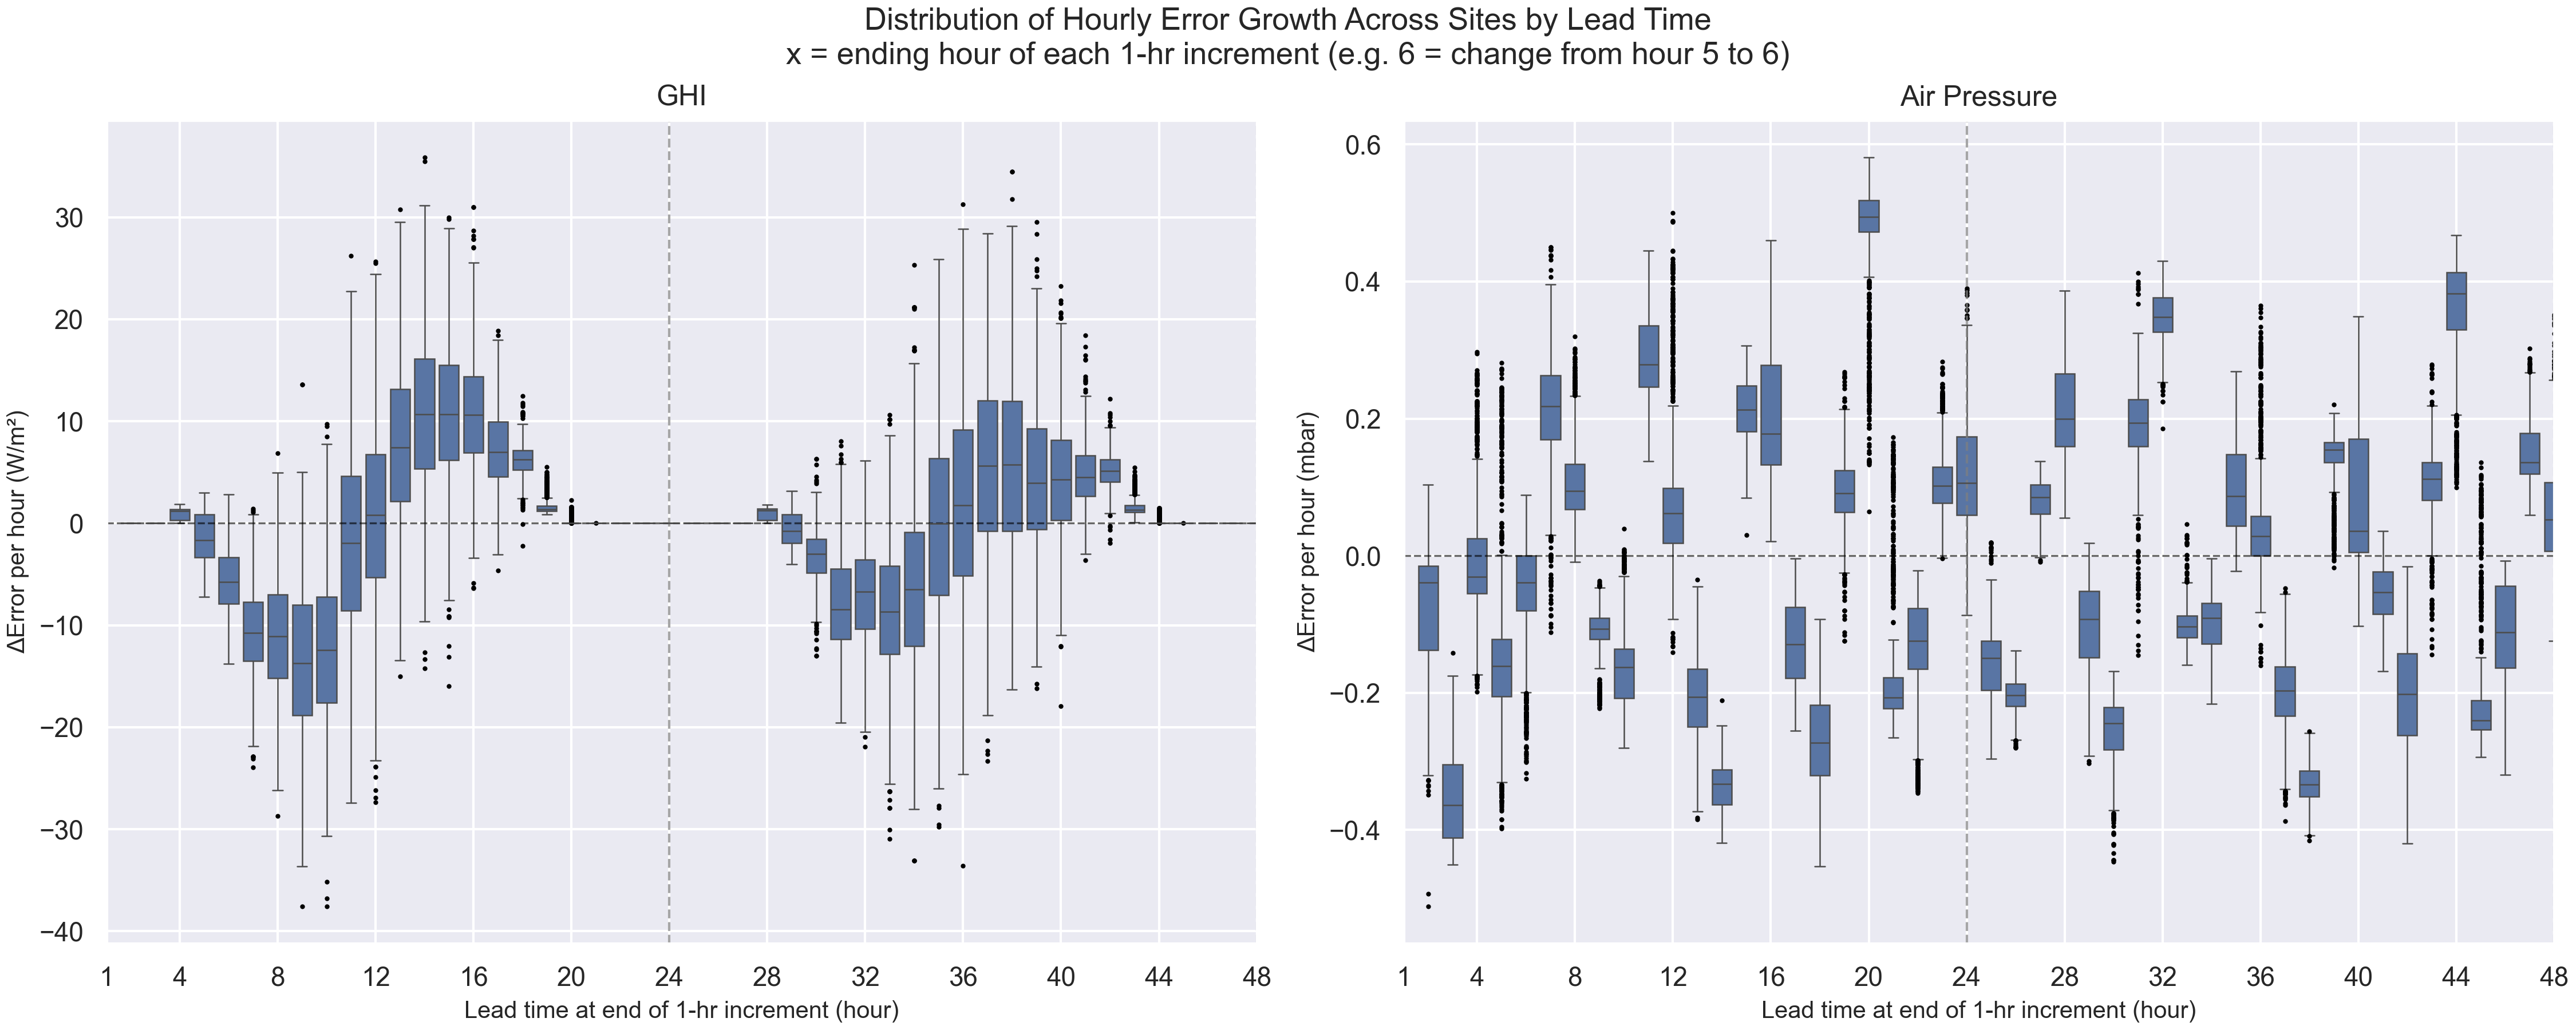
\includegraphics[width=\textwidth]{figures/Q2/embed/error_growth_distributions_ghi_pressure copy.png}
  \caption{Distribution of the hourly error-growth rate ($\Delta\text{Error}/\text{hr}$) across
  all \num{896} sites at each lead time, one boxplot per lead hour and one panel per variable.
  GHI shows the diurnal sinusoid in its box centres with visibly larger spread during the day;
  the other variables stay centred near zero with roughly constant spread across lead time,
  indicating that error-growth volatility does not systematically increase further out. Pressure
  has the widest boxes (most volatile across sites).}
  \label{fig:growthdist}
\end{figure}

As shown by these plots, GHI has the most prominent sinusoidal pattern with a 24-hr cycle, but a few other weather variables hint at this as well, such as relative humidity. Furthermore, it seems that for all variables the error growth rate is centered at 0 across all lead times. These observations warranted statistical tests to evaluate their significance.

\subsection{Statistical testing}

We ran two tests to assess the significance of these two findings. Multiple-comparison control uses
the Benjamini--Hochberg FDR procedure throughout.

\begin{description}
  \item[Test 1 --- Harmonic / diurnal cycle.] We fit the error growth to a harmonic regression,
        $\text{growth}(h) = A\sin(2\pi h/24) + B\cos(2\pi h/24) + C$, and used permutation tests
        on the amplitude. After FDR correction, the amplitudes for \textbf{GHI, RH, U10, and
        wind direction} are statistically significant, supporting a genuine 24-hour cycle in
        those variables.
  \item[Test 2 --- Bias drift.] A Wilcoxon test for a systematic bias shift across the horizon
        found \emph{no} variable with a statistically significant drift---error growth does not
        lean consistently positive or negative.
\end{description}

\begin{figure}[H]
  \centering
  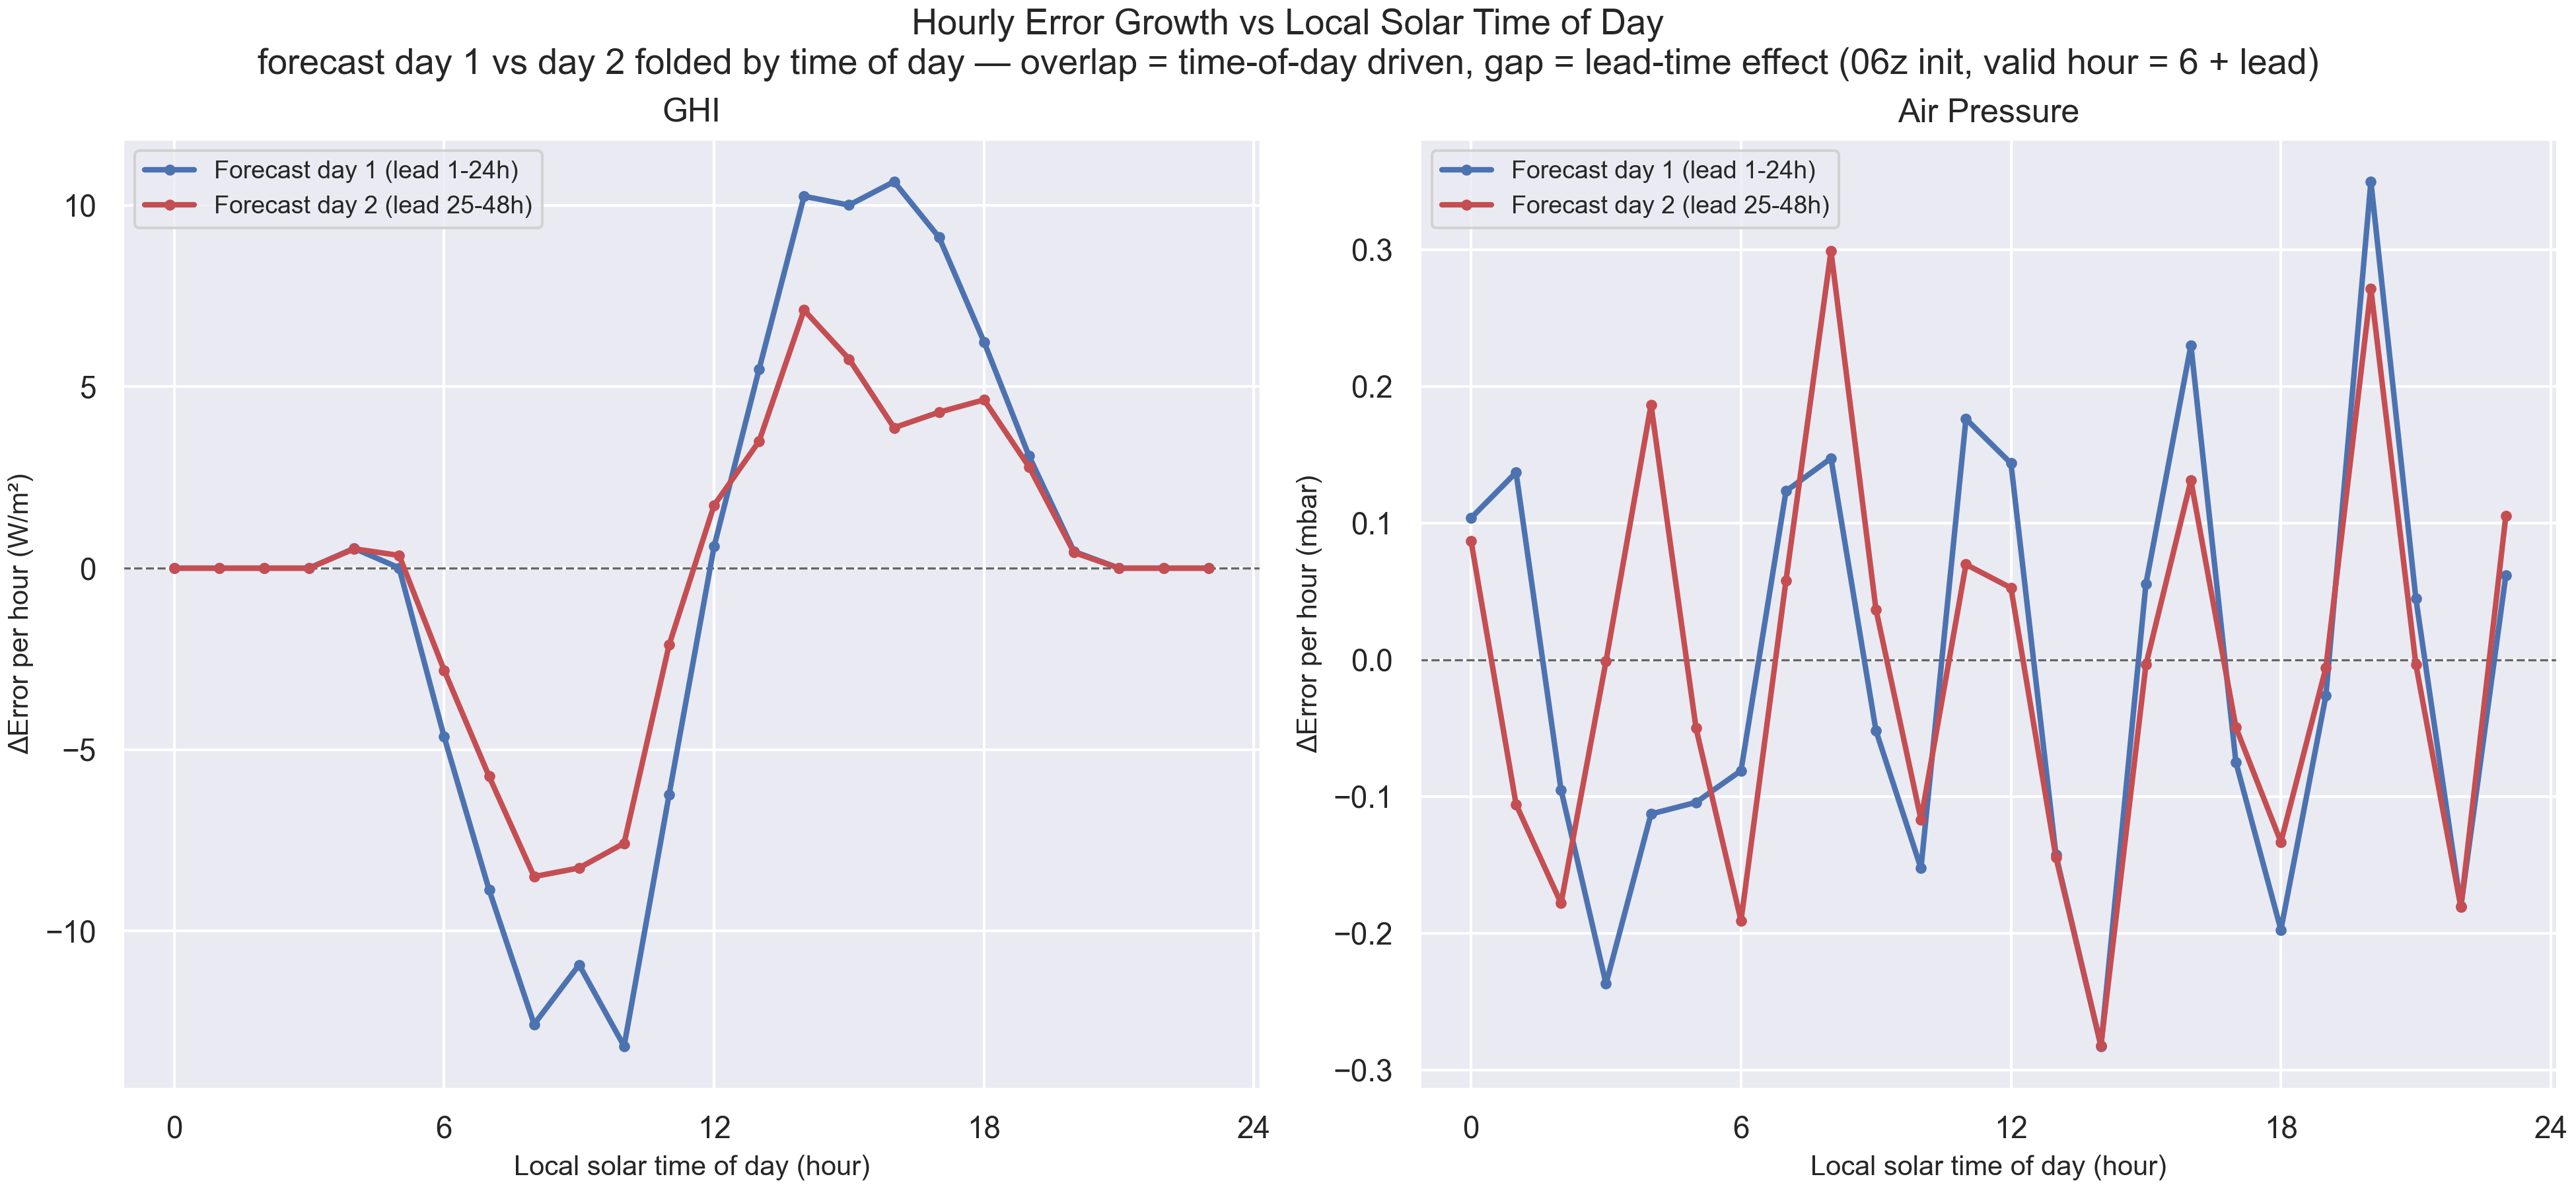
\includegraphics[width=\textwidth]{figures/Q2/embed/error_growth_tod_ghi_pressure copy.png}
  \caption{Hourly error growth folded onto local solar time of day, with forecast day~1
  (leads 1--24~h) and day~2 (leads 25--48~h) overlaid. Because lead $h$ and lead $h{+}24$ land
  at the same time of day, overlapping lines indicate a purely time-of-day signal, while a
  vertical gap would indicate a genuine lead-time effect. The two days track closely for most
  variables, confirming the growth pattern is time-of-day driven.}
  \label{fig:tod}
\end{figure}

\subsection{Implications}

Forecast errors are largest at lead times of 12--16 and 36--40 hours, so day-ahead grid
scheduling at those horizons carries the most uncertainty. Since MAE and RMSE gradually rise and have a widening gap across lead times and RMSE weighs larger errors more, larger errors are more frequent for longer lead times. This implies taht forecast stability drops as lead time goes up. Because error growth centers on zero
for every variable, scheduling is not expected to systematically over- or under-commit. Most
usefully, the significant 24-hour cycle in GHI, RH, U10, and wind direction is \emph{correctable}:
one can model the bias as a function of time of day with harmonic regression and subtract it from
the forecast.
